
\bibliographystyle{asp2010}

\markboth{Wu et al.}{The MWA Archive}

\title{The MWA Archive - A Multi-tiered Dataflow and Storage System}
\author{Che~ Wu,$^1$ Andreas~Wicenec,$^1$ Dave~Pallot,$^2$ and Alessio~Checcucci$^1$
\affil{$^1$ICRAR/University of Western Australia}
\affil{$^2$ICRAR/Curtin University}}

\aindex{Wu, C.}
\aindex{Wicenec, A.}
\aindex{Pallot, D.}
\aindex{Checcucci, A.}

\begin{abstract}
The Murchison Widefield Array (MWA) is a next-generation radio telescope, generating visibility data products continuously at about 400 MB/s. The entire MWA archive consists of dataflow and storage sub-systems distributed across three tiers.
\end{abstract}


\section{MWA Data Products}
The Murchison Widefield Array (MWA) is optimized for the observation of extremely wide fields at frequencies between 80-300 MHz. 
The complete array will provide about 2000 $m^2$ of collecting area at 150 MHz with 30.72 MHz instantaneous bandwidth at 40 kHz spectral resolution and a field of view between 200 and 2500 square degrees with a time resolution of 0.5 seconds. The initial MWA commissioning will install 32 antennae referred to as ``tiles". Each tile is a 4 by 4 grid of dual-linear-polarization, wide-beamwidth antenna elements. Each data sample is a complex number representing the amplitude and phase of a signal at a particular point in time within a specific frequency channel. For each channel at each time step, the correlator carries out \((N \times (N + 1) / 2) \times (2  \times 2) = 2N(N+1) \) pair-wise cross/auto-correlation, where \(N\) denotes the number of tiles, and \(2 \times 2 \) indicates that polarised samples of orthogonal directions are cross-correlated. For example,  under the \(N=32\)-tile configuration during commissioning, each correlator produces \(2,112\) visibilities per frequency channel per time step. Since a ``visibility" is a complex number (\(2 \times 32\) bits \(= 8\) Bytes), the aggregated data rate amounts to \( 2N(N+1) \times 8 \times 1/T \times M\) per second, where \(T\) denotes the time resolution (i.e. 0.5 seconds). \(M\) is the total number of frequency channels: \(30.72\) MHz bandwidth \(/\) \(40\) kHz spectral resolution \(= 768\). Hence correlators under the full 128-tile configuration will produce visibility data at \(387\) MB/s. This requires 24 on-site GPU-based software correlators, each processing 32 channels, and producing frequency-split visibilities at a rate of about \(16\) MB/s. 

During the 32-Tile phase of the MWA commissioning, two GPU machines with software correlators have been deployed at MRO. For the purpose of commissioning, the spectral resolution is set to 10kHz with a 1-second time resolution. Therefore, each one of the two correlators shares 30.72 MHz \(/\) 10kHz \(/\) 2 = 1,536 frequency channels, generating visibilities at the rate of \(24.75\) MB/s. Visibilities are currently stored, along with several observation-specific metdata, as FITS image or binary table extensions. In addition to visibilities, it is envisaged that images produced by the real-time imaging pipeline \citep{ord2010interferometric} running on those GPU boxes will also be archived online.

   \begin{figure}
   \begin{center}
   \begin{tabular}{c}
   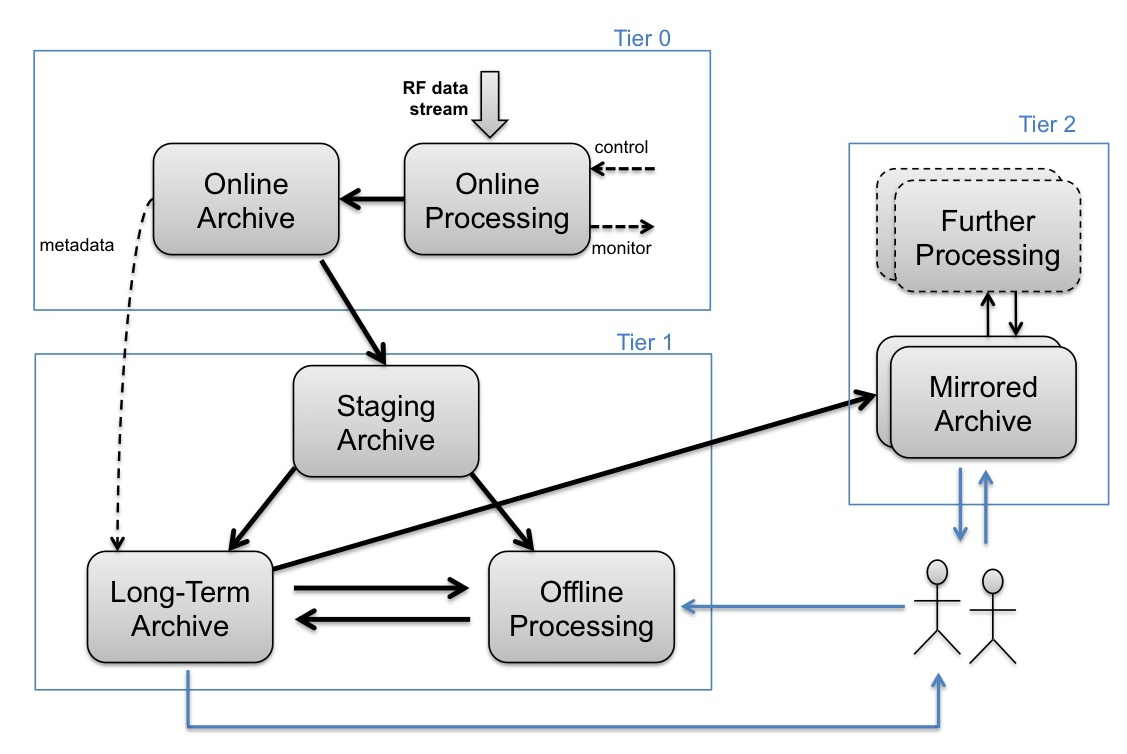
\includegraphics[height=8cm]{part6/Wu_P34/P34_f1.eps}
   \end{tabular}
   \end{center}
   \caption[example] 

   { \label{fig:con_dataflow} 
MWA Archive - Conceptual Dataflow}
   \end{figure} 

\section{Conceptual Dataflow}
The conceptual dataflow (see Figure~\ref{fig:con_dataflow}) consists of three tiers. Tier 0 is co-located onsite with the telescope, consisting of the \emph{Online Processing} system and the \emph{Online Archive} system. The software correlator and the DataCapture are part of the ``real-time" \emph{Online Processing} system. Radio-frequency voltage samples are collected from antennae by the receiver, which generates digitized streams at an aggregated rate of 320 Gb/s to the Correlator. The Correlator produces visibilities that are captured by the \emph{DataCapture}, which generates format/product-specific ``observation splits" before pushing them to the \emph{Online Archive}. For visibility products, frequency-split FITS extension files are archived at Tier 0.

   \begin{figure}
   \begin{center}
   \begin{tabular}{c}
   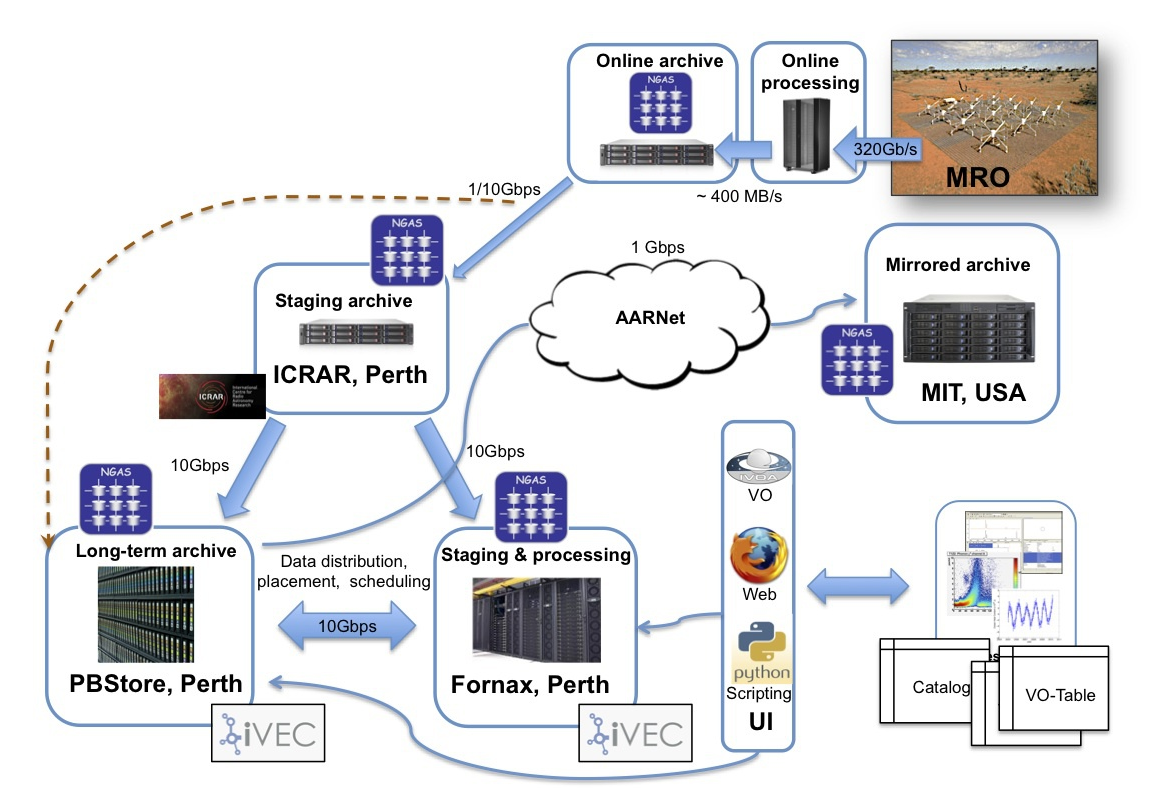
\includegraphics[height=9cm]{part6/Wu_P34/P34_f2.eps}
   \end{tabular}
   \end{center}
   \caption[example] 

   { \label{fig:phy_dataflow} 
MWA Archive - Physical Dataflow}
   \end{figure} 

The \emph{Online Archive} at Tier 0 periodically transfers captured data to \emph{Staging Archive} at Tier 1 through Wide Area Networks (WAN), and recycles its local archival storage for subsequent observations. Meanwhile, metadata on instruments, observations, and monitor \& control are also periodically synchronised from the \emph{Online Archive} directly to the\emph{Long-term Archive} via WAN. Data at Tier 1 is always delivered directly to the \emph{Long-term Archive} at a high priority.  In addition, another copy will be sent to the \emph{Offline Processing} for (re-)processing, such as reduction, calibration, transformation, imaging, etc. before the data products can be used for science. The \emph{Offline Processing} at Tier 1 will push reduced data products to the \emph{Long-term Archive} before recycling its storage for the next batch of data streams from Tier 0. Upon user requests, the \emph{Offline Processing} may retrieve data from the \emph{Long-term Archive} for re-processing (e.g. using different algorithms or parameters) and archives the results back to the \emph{Long-term Archive}. From there, more copies will be selectively delivered to sets of the \emph{Mirrored Archives} at Tier 2 that have subscribed themselves to data products of their own research interests. The \emph{Mirrored Archive} facilities host a subset of the data products in remote sites and provide local processing capabilities for their scientists to further reduce and analyze the data. Scientists can access data products from either Tier 1 or Tier 2 based on their geographic locations and research projects. Optimized data placement strategies based on user access patterns are essential to avoid unnecessary data transfer and storage activities.


\section{Physical Dataflow and Storage}
The physical dataflow (see Figure~\ref{fig:phy_dataflow}) realizes the conceptual dataflow with physical network links and archival storage systems. At Tier 1 in MRO, the \emph{Online Processing} has been implemented in software running on a 24 iDataplex dx360 GPU node GPU cluster connected via two Ethernet networks for data and meta-data respectively. To meet the 387MB/s bandwidth requirement, the data network uses a 10G Ethernet switch, which connects GPU nodes to the \emph{Online Archive}. The hardware of both the \emph{Online Archive} and the \emph{Staging Archive} is a Supermicro node with 4 quad-core 2.40 GHz Intel Xeon CPUs, 32GB of memory, and a 10Gb Ethernet network host adapter. The storage attached contains 12 SAS HDD (providing a total of 20 TB) configured as RAID5. The link between MRO and Perth is connected through a dedicated fibre network link with the city of Geraldton (350 km south-east the MRO). From there, via the Australian National Broadband fibre network, it is connected to the Pawsey High Performance Computing (HPC) Centre in Perth. Initially the long-distance link will only provide a 1 Gbit/s bandwidth, but will be upgraded to 10 Gbit/s to accommodate the full MWA data rate.

The Next Generation Archive System (NGAS) software layer is deployed for data management on all archival facilities (Online, Staging, Mirrored, and Long-term). Originally developed at ESO \citep{wicenec2007eso}, NGAS has been used in several observatories including ALMA \citep{wicenec2004alma} and the NRAO to archive and host data. NGAS manages registering, checking data, and possibly replicating data to another storage location as fast as possible in order to secure it against loss. More importantly, NGAS allows customization that adapts itself to data ingestion with different formats and throughput requirements (e.g. MWA). NGAS is flexible enough to adjust itself to the hardware and deployment environment required. For example, NGAS supports the mixed network and media transport requirement during the early operational phases of the telescope. NGAS is also able to take full advantage of different types of archival storage mediums through its data archive plugin framework.

The \emph{Long-term Archive} is implemented as NGAS servers atop of the SUN (Oracle) StorageTek SAM storage and archive management software installed at the Cortex PBStore environment as part of the Pawsey HPC Centre. Essentially, this Hierarchical Storage Management (HSM) system archives data by copying files from the online disk cache (i.e. DDN disk arrays) to the archive media (i.e. tape volumes), stages data by moving files from tape volumes back to the disk cache on retrieval demand, releases data by removing files from the disk cache according to data policies, and finally recycles data by reclaiming space occupied by unused (e.g. dated versions) file copies from the archive media. The key challenge is to integrate this HSM system into our NGAS data management framework in order to strike a balance between storage capacity and access latency based on MWA user access patterns. In particular, the handling of retrieval / re-processing requests to tape-resident data should mask the slow ``staging" phase from the archive media to the disk cache. To address this issue, techniques such as asynchronous data access, data prefetching, and optimized data placement are being integrated into the NGAS archive plugin framework.  

Our previous disk-based archiving throughput tests \citet{wiceneca2012mwa} suggested that the aggregated disk transfer rate reached 400 MB/s on a single disk array managed by multiple NGAS instances. Our network experiment also shows that the maximum transfer rate from Perth to MIT (Cambridge, USA) using multiple concurrent TCP streams is 900 Mbits/s, which is far less than the disk transfer rate. Hence, we deployed a multi-threaded concurrent file transfer mechanism in the existing NGAS data subscription framework to implement the data delivery from \emph{Long-Term Archive} to \emph{Mirrored Archive}. We also developed a subscription filter plugin that filters out data unrelated to research projects conducted at MIT. Current work-in-progress includes HSM data prefetching, data access pattern analysis, archival storage benchmarking, and the MWA science database development.

\bibliography{editor}
